% !Mode:: "TeX:Hard"
\documentclass{article}
\usepackage{amsmath,amsthm}
\usepackage{amsfonts}
\usepackage{a4wide}

% This is to tune using tiks with tex4ht
\ifdefined\HCode
   \def\pgfsysdriver{pgfsys-dvisvgm4ht.def}
\fi
%%%%%%%%%%%%%%%%%%%%%%%%%%%%%%%%%%%%%%%%%
\usepackage{tikz}
\usetikzlibrary{shapes,arrows,positioning,fit}


\title{My notes on how to use Tex4ht+MathJax}
\author{Victor Kozyakin}

%\usepackage{tex4ht}
\begin{document}
\maketitle

\section{Call Command}\label{S1}
My problem was to make a HTML file with plenty of mathematics from a \LaTeX{}
one. As a beginner, I immediately faced the following problems:
\begin{itemize}
  \item How to run Tex4ht to get HTML file with mathematics?
  \item What to do to make proper referencing of mathematical formulas?
  \item How to cope with TikZ figures?
\end{itemize}

After a while I discovered that the most suitable way for me is to join
Tex4ht with MathJax. And the simplest way was to run the following command to
process \verb|test.tex| file:

{\small
\begin{verbatim}
make4ht -s test.tex "myconfig" " -cunihtf -utf8"
\end{verbatim}}
\noindent and after that, if one wants to embed into resulted
\verb|test.html| the css-file \verb|test.css| generated during previous
command, one should issue one the following command {\small
    \begin{verbatim}
htlatex test.tex "myconfig" " -cunihtf -utf8"
\end{verbatim}
    \noindent or once more
    \begin{verbatim}
make4ht -s test.tex "myconfig" " -cunihtf -utf8"
\end{verbatim}}
\noindent where the config file \verb|myconfig.cfg| is as
follows

  {\small
    \begin{verbatim}
\Preamble{xhtml,html5,0,mathjax,p-indent,charset=utf-8,css-in,fn-in}
\textwidth=2160pt

\Css{body { margin:5\% 5\%; max-width:72em; font-size:large; padding:0 40px;}}
\Css{p.indent {text-indent:1.5em;}}
\Css{.columns-3 p.indent {text-indent:0em;}}
\Css{p.bibitem-p { text-indent: 1.5em; margin-left: 2em; margin-top:0em; margin-bottom:0em;
    background:\#F0F0F0; color:\#000000;}}

\Configure{@HEAD}{\HCode{
<script>
window.MathJax = {
  tex: {
    tags: "ams",
    processEscapes: true,
    processEnvironments: true,
    packages: ['base', 'color', 'ams', 'boldsymbol', 'newcommand', 'verb']
  },
  loader: {
    load: ['[tex]/color', '[tex]/ams', '[tex]/boldsymbol', '[tex]/newcommand', '[tex]/verb']
  }
};
</script>\Hnewline
}}

\def\eqref#1{$\mathrm{(\ref{#1})}$}

\begin{document}

\EndPreamble
\end{verbatim}}

\section{How to reference equations in TeX4ht+MathJax}\label{S2}
Unfortunately, it turned out that reference in conjunction TeX4ht+MathJax
works well when they referenced sections, subsections and other structure
element that are in \textbf{text mode}, but when you are trying to reference
the label of equation you are getting ???.

The problem is turned out to be rather easily solvable: to reference labels
of equations, align or other things in \textbf{math mode} you should put the
calling \verb|\eqref| or \verb|\ref| in a \textbf{math environment}, e.g. by
surrounding them by \verb|$'s| or \verb|\(|\ldots\verb|\)|. Another way is to
redefine the command \verb|\eqref| in order that it will be invoked in math
mode automatically (see the appropriate string in the config file
\verb|myconfig.cfg|.

So, for the \LaTeX{} code below
  {\small
    \begin{verbatim}
\begin{equation}
\boldsymbol{f}(x)=1\label{eq}
\end{equation}

\[
1\neq1. \tag{OneIsNotOne Condition}\label{E:mycond}
\]

Here, the reference to \tag{OneIsNotOne Condition} in previous
equation is as follows: \eqref{E:mycond}

\begin{align}
a&=1\label{A}\\
b&=0\label{B}
\end{align}
Example of references: we have equation \eqref{eq} from Sec. \ref{S1}. Or $\ref{A}$-\eqref{B}.
\end{verbatim}}
\noindent we obtain the following output:

\begin{equation}
  \boldsymbol{f}(x)=1\label{eq}
\end{equation}

\[
  1\neq1. \tag{OneIsNotOne Condition}\label{E:mycond}
\]

Here, the reference to \verb|\tag{OneIsNotOne Condition}| in previous
equation is as follows: \eqref{E:mycond}

\begin{align}
  a & =1\label{A} \\
  b & =0\label{B}
\end{align}
Example of references: we have equation \eqref{eq} from Sec. \ref{S1}. Or
$\ref{A}$-\eqref{B}.

\section{How to cope with TikZ figures}\label{S3}
Tex4th supports TikZ, however, for correct displaying text and math symbols
in TikZ picture, it is needed to put in the preamble of tex file the
following lines, before TikZ package loading:
\begin{verbatim}
\ifdefined\HCode
   \def\pgfsysdriver{pgfsys-dvisvgm4ht.def}
\fi
\end{verbatim}

Below is an example of using TikZ.

\begin{figure}[!hbt]
  \center
  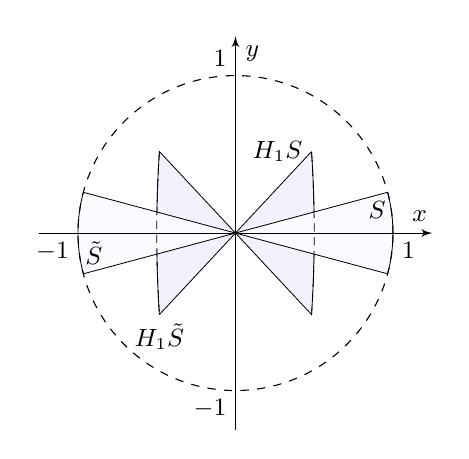
\begin{tikzpicture}[auto,>=latex',node font=\small]
    \pgfmathsetmacro{\a}{15}
    %
    \begin{scope}[xscale=0.5, yscale=2.0]
      \pgfmathsetmacro{\s}{2}
      \coordinate (S) at ({cos(\a)*\s},{sin(-\a)*\s});
      \coordinate (SS) at ({cos(\a)*\s},{sin(\a)*\s});
      \draw[fill=blue!5, line width=0.3pt] (SS) to (0,0) to (S) arc [start angle=-\a, end angle=\a, radius=\s];
      \path (SS) node[left] {$H_{1}S$};
    \end{scope}
    %
    \begin{scope}[xscale=-0.5, yscale=-2.0]
      \pgfmathsetmacro{\s}{2}
      \coordinate (S) at ({cos(\a)*\s},{sin(-\a)*\s});
      \coordinate (SS) at ({cos(\a)*\s},{sin(\a)*\s});
      \draw[fill=blue!5, line width=0.3pt] (SS) to (0,0) to (S) arc [start angle=-\a, end angle=\a, radius=\s];
      \path (SS) node[below] {$H_{1}\tilde{S}$};
    \end{scope}
    %
    \pgfmathsetmacro{\s}{2}
    \coordinate (S) at ({cos(\a)*\s},{sin(-\a)*\s});
    \coordinate (SS) at ({cos(\a)*\s},{sin(\a)*\s});
    \draw[fill=blue!2, line width=0.3pt] (SS) to (0,0) to (S) arc [start angle=-\a, end angle=\a, radius=\s];
    \path (SS) node[below left,xshift=0.66ex] {$S$};
    %
    \begin{scope}[scale=-1.0]
      \pgfmathsetmacro{\s}{2}
      \coordinate (S) at ({cos(\a)*\s},{sin(-\a)*\s});
      \coordinate (SS) at ({cos(\a)*\s},{sin(\a)*\s});
      \draw[fill=blue!2, line width=0.3pt] (SS) to (0,0) to (S) arc [start angle=-\a, end angle=\a, radius=\s];
      \path (SS) node[above right,xshift=-0.66ex] {$\tilde{S}$};
    \end{scope}
    %
    \begin{scope}[xscale=0.5, yscale=2.0]
      \pgfmathsetmacro{\s}{2}
      \coordinate (S) at ({cos(\a)*\s},{sin(-\a)*\s});
      \draw[densely dashed, line width=0.3pt] (S) arc [start angle=-\a, end angle=\a, radius=\s];
    \end{scope}
    %
    \begin{scope}[xscale=-0.5, yscale=-2.0]
      \pgfmathsetmacro{\s}{2}
      \coordinate (S) at ({cos(\a)*\s},{sin(-\a)*\s});
      \draw[densely dashed, line width=0.3pt] (S) arc [start angle=-\a, end angle=\a, radius=\s];
    \end{scope}
    \draw[->] (-\s-0.5,0) -- (\s+0.5,0) node[label={[xshift=-0.5em,yshift=-0.66ex]$x$}] {};
    \draw[->] (0,-\s-0.5) -- (0,\s+0.5) node[label={[xshift=0.66em,yshift=-4ex]$y$}] {};
    %
    \draw[dashed] (0,0) circle [radius=\s];
    \node[above left] at (0,\s) {$1$};
    \node[below left] at (0,-\s) {$-1$};
    \node[below right] at (\s,0) {$1$};
    \node[below left] at (-\s,0) {$-1$};
  \end{tikzpicture}
  \caption{Example of Stanford}
\end{figure}

Citation example:~\cite{NDKKP:DSS96}

\newcommand{\BibAnnote}[1]{}%
\bibliographystyle{ugost705s}
\bibliography{kozpub}

\end{document}

% make4ht -sc myconfig.cfg test.tex "0,mathjax,p-indent,charset=utf-8" " -cunihtf -utf8"
